\chapter{INTRODUCTION} \label{ch:introduction}

The construction of optical circuits and systems is a complex and expensive process. Engineers invest substantial resources in the design and fabrication of a circuit. Given the scale and expense involved in realizing even the simplest system, it is necessary to model or simulate circuits before fabrication in order to validate designs and ensure that they meet project requirements.

While many simulation techniques exist, this paper focuses on the finite-difference, time-domain (FDTD) method and its implementation. 

Although conceptually simple, FDTD in large scale requires significant computational resources in order to facilitate a quick, iterative design process. One way to address this challenge is employ clusters of powerful computers. By distributing a simulation across a cluster, capabilities may be scaled in two ways. The increased memory makes it possible to solve larger problems which may not fit within the relatively limited resources available on a single machine. Increased processing power reduces the amount of time that is required to solve a given problem.

While effective, this approach presents several challenges. Provisioning of clusters of powerful computers is an expensive proposition, and may strain or exceed the budgets of smaller organizations. Even within institutions which posses the required compute resources, high demand for access to said resources may present a bottleneck, again slowing the iterative design process which this approach was intended to solve.

Another approach, which has not gained adoption among FDTD software providers, is the use of graphics processing units (GPUs) to solve highly parallelizable problems. While a relatively new field of study, the applicationn of GPUs to general computing problems as promising, and has already yielded impressive results in areas such as medical research, machine learning, artificial intelligence and others. 

This paper explores a GPU-based implementation of FDTD and examines it's performance relative to existing CPU-based implementations. 



 



\section{Homogeneous Isotropic Turbulence}

The governing equations are the incompressible Navier Stokes equations:
\begin{eqnarray}
    \frac{\partial\textbf{u}}{\partial t} + (\textbf{u}\cdot\nabla)\textbf{u} & = & -\frac{1}{\rho}\nabla p + \nu \nabla^2\textbf{u} + \textbf{F}, \\
    \nabla \cdot \textbf{u} & = & 0 , \label{eq: intro navier stokes}
\end{eqnarray}
where $\textbf{u}$ is the flow velocity, $\rho$ is the fluid density, $p$ is the pressure, $\nu$ is the kinematic viscosity, and $\textbf{F}$ is the forcing. The density is constant so there are no buoyancy effects. The viscosity is also constant.  Moreover, the fluid is unbounded so there are no walls and boundary layers.  We consider an idealized forcing specified in wave number space at a single spatial frequency so that we have homogeneity and isotropy.  Under these circumstances we can transform the entire problem to Fourier space.  There, a single equation describes the problem:
\begin{equation}
    \left(\frac{\partial}{\partial t} + \nu k^2\right)\hat{u}_i\left(\vec{k},t\right) = -ik_mP_{ij}\left(\vec{k}\right)\int_{\vec{p}+\vec{q} = \vec{k}}\hat{u}_j(\vec{p},t)\hat{u}_m(\vec{q},t)d\vec{p} + \hat{F}_i(\vec{k}), \label{eq: intro spectral navier stokes}
\end{equation}
where $\hat{u}$ is the Fourier transform of $u$, $\hat{u}_i$ is the $i$-component of the Fourier velocity vector, $k$ is the wave number, $\hat{F}$ is the Fourier transform of the forcing, $\vec{k}$, $\vec{p}$ and $\vec{q}$ are wave vectors
\begin{equation}
    P_{ij}\left(\vec{k}\right) = \delta_{i,j} - \frac{k_ik_j}{k^2}
\end{equation}
is the projection operator that removes the pressure term.  This is the traditional starting point for the study of homogeneous isotropic turbulence \cite{Batchelor, Hinze, McComb} which always develops when the forcing is strong enough to give a high Reynolds number.

Homogeneity and isotropy refers to independence of location and orientation in space. The first to utilize this type of turbulence was G.I. Taylor \cite{Taylor1935}. With these properties it makes sense to talk about energy per unit volume, e.g.
\begin{equation}
    E = \frac{1}{2}\langle |\vec{u}|^2 \rangle_{\mbox{unit box}}.
\end{equation}
where $\langle \dot \rangle$ means average and unit box is defined as $[0,1]$ by $[0,1]$ by $[0,1]$.
It is traditional to decompose the energy according to the wave number in Fourier space.  This gives the energy spectrum $E(|\vec{k}|)$ which is typically plotted on double logarithmic scales as sketched in Figure \ref{fig: intro energy spectrum}.
\begin{figure}[!htp]
    \begin{center}
   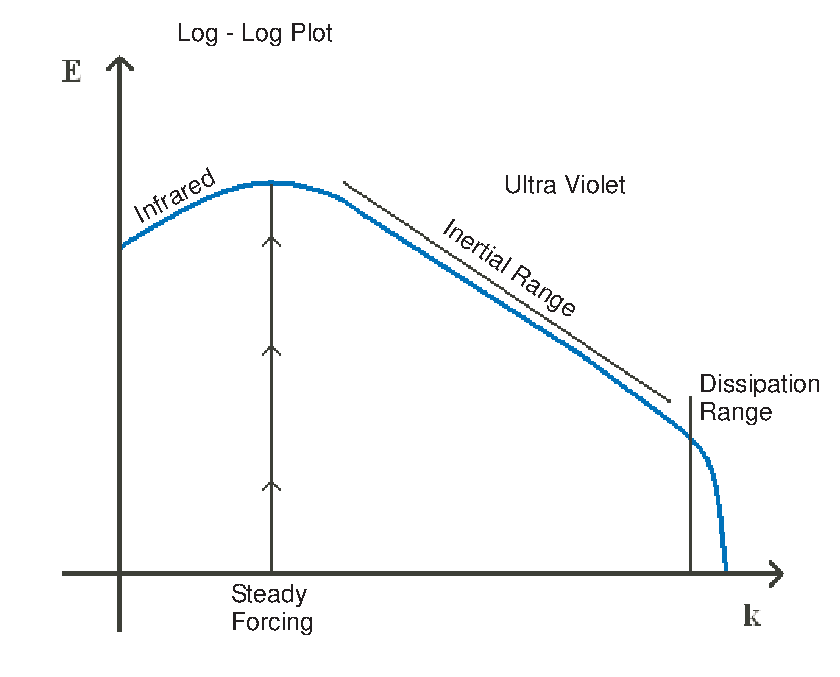
\includegraphics[width=4in]{intro_energyspectrum.eps}
   \end{center}
  \caption{Sketch of an energy spectrum. (eps file)} \label{fig: intro energy spectrum}
\end{figure}
The reason for using the double logarithmic scales is that some parts of the spectrum obey power laws and thus become straight lines in Figure \ref{fig: intro energy spectrum}.  In particular, the inertial range obeys a power law with slope $-5/3$ or nearly so.  The $-5/3$ value was obtained theoretically by Kolmogorov 1941 via a scaling argument together with his four-fifth's law \cite{Kolmogorov}.  Experimental evidence \cite{Frisch, Grant, Champagne} has confirmed an inertial range with slope near $-5/3$.

\section{Moments of the Inertial Range}

To study the inertial range, moments of various quantities are employed.  The energy spectrum is just one example of an inertial range moment obeying a power law; other examples include $\langle |\hat{u}(\vec{k})|^p\rangle$.  There is a transform specifically designed to deal with moments, namely, the Mellin transform.  It is related to the more familiar Fourier and Laplace transform through various manipulations in the complex plane; see \cite{Sneddon}.

\subsection{Mellin Transforms}

The Mellin transform is defined as
\begin{equation}
      \Phi(z) = \mathcal{M}[\phi(x);z] \equiv \int_{0}^{\infty}x^{z-1}\phi(x)\ dx. \label{eq:mellin}
\end{equation}
When $\phi(x)$ is a probability density function of a \emph{positive} random variable $X$,
\begin{equation}
    \phi(x)dx = Pr\{x<X<x+dx\}, \quad x>0,
\end{equation}
then the moments of $X$ are
\begin{equation}
    \langle X^{p}\rangle = \int^{\infty}_{0}x^{p}\phi(x)dx.
\end{equation}
Next, we introduce $x$ into the equation so that we may write moments in terms of Mellin transforms;
\begin{eqnarray}
    & = & \int^{\infty}_{0}x^{p+1}\phi(x)\frac{dx}{x} \nonumber \\
    & = & \mathcal{M}[\phi(x);p+1]. \label{eq: moments of chi}
\end{eqnarray}
Since the random variable is positive, moments of non-integer orders are readily defined\footnote{We can also use Mellin transforms for a random variable that is only real rather than positive.   To do this, we split $\phi$ unto its odd and even parts.  Each part can then be treated similarly to (\ref{eq: moments of chi}).}.  The only restriction on $p$ is that the improper integral must converge.  The function $\phi$ is then uniquely determined from its moments through the inverse Mellin transform. It, like the inverse Laplace transform, involves a contour integral in the complex plane.

In order to use the Mellin transform in our investigations, it is necessary that we know how various self-similarities transform.  Suppose, our pdf, $\phi$, depends parametrically on a length scale, $\ell$, i.e. $\phi = \phi(x,\ell)$, in a self-similar way where $\ell = 2\pi/k$.  For example, we could have
\begin{equation}
    \phi(x,\ell) = C(\ell)f\left( \frac{x}{\sigma(\ell)}\right), \label{eq: self similar ex}
\end{equation}
where $\sigma = \langle X^{2}\rangle^{1/2}$ and $f(x) \geq 0$, represents the similarity profile.  Of course, $C$ would then be specified by the requirement that $\phi(x,\ell)$ be a pdf, i.e.
\begin{eqnarray}
    \int^{\infty}_{0}\phi(x,\ell)dx = & C\int^{\infty}_{0}f\left(\frac{x}{\sigma(\ell)}\right)dx & = 1 \\
    \Rightarrow C = & \left( \sigma\int^{\infty}_{0}f(u)du\right)^{-1} & = \sigma^{-1}.
\end{eqnarray}
For the Mellin transform, we then have
\begin{eqnarray}
    \mathcal{M}[\phi(x;\ell);z] & = & C\mathcal{M}\left[f\left(\frac{x}{\sigma}\right);z \right] \nonumber \\
    & = & C\sigma^{z}\mathcal{M}[f(x);z] \nonumber \\
    & = & \sigma^{z-1}\frac{F(z)}{F(1)}
\end{eqnarray}
where $F(z) = \mathcal{M}[f(x);z]$ and $F(1) = 1$ only if $f(x)$ is a pdf.

Correspondingly, we have
\begin{equation}
    \langle X^{p} \rangle = \mathcal{M}[\phi(x;\ell); p+1] = \frac{\sigma^{p}(\ell)F(p+1)}{F(1)}
\end{equation}
and
\begin{equation}
    \langle X \rangle^{p} = \mathcal{M}[\phi(x;\ell); 2]^{p} = \left(\frac{\sigma(\ell)F(2)}{F(1)}\right)^{p},
\end{equation}
so that the dimensionless ratio
\begin{equation}
    \frac{\langle X^{p} \rangle}{\langle X \rangle^{p}} = \frac{F(p+1)}{F(1)}\left(\frac{F(2)}{F(1)}\right)^{p} \label{eq: dimensionless ratio}
\end{equation}
is independent of $\ell$.  The self-similarity (\ref{eq: self similar ex}), also known as global scaling invariance or statistical self-similarity, was used by Kolmogorov as a postulate in his 1941 theory to obtain the $-5/3$ slope \cite{Kolmogorov}. From (\ref{eq: dimensionless ratio}) it follows that the corresponding exponents are linear, i.e. if $\langle X^{p}\rangle = C_{p}\ell^{\zeta_{p}}$ then $\zeta_{p} = p\zeta_{1}$.

\section{Scaling Exponents}

In the inertial range, the moments of almost any numerical value one can think of are power laws in the scale.  When working in Fourier space the magnitude of the wave number $|\vec{k}|$ defines the scale.  However, not all theoretical investigations use Fourier space.  The Karmon-Howarth equation \cite{Hinze}, for example, works with a spatial length scale.  This equation, formulated in the thirties, uses two point spatial correlations for the reason that these are readily obtained experimentally.  Specifically, velocity differences between two points depend only on the separation distance $\ell$ when the turbulence is homogeneous and isotropic.  Only two velocity differences come into play: $\delta v_{\parallel}(\ell)$ and $\delta v_{\perp}(\ell)$.  The former is parallel to the line segment connecting the two points, the latter perpendicular to it.  For the second order moments, e.g. $\langle (\delta v_{\parallel})^2\rangle$, a direct connection can be established with Fourier space through Parseval's identity.  For other orders there is, unfortunately, no similar connection.

The four-fifth's law of Kolmogorov in 1941 was formulated in terms of $\delta v_{\parallel}(\ell)$.  This states
\begin{equation}
    \langle (\delta v_{\parallel})^3\rangle = -\frac{4}{5} \epsilon \ell
\end{equation}
where $\epsilon$ is the dissipation. Combining the four-fifth's-law with the assumption of statistical self-similarity (\ref{eq: self similar ex}), he readily obtained
\begin{equation}
    \langle (\delta v_{\parallel})^p\rangle = C_p\ell^{\zeta_p} = \tilde{C}_p\epsilon^{p/3}\ell^{p/3}
\end{equation}
with $\zeta_p = \zeta_3\dot p/3 = p/3$, where $C_p$ are supposedly universal coefficients.  This scaling law is commonly called K41.  Note $\zeta_p$ is a linear function of $p$.  The -5/3 slope of the energy spectrum is a direct consequence of K41.  The idea of universal coefficients soon was questioned by Landau \cite{Frisch}.  Since the sixties it also has become clear that the scaling exponents $\zeta_p$ are nonlinear, which is referred to as anomalous scaling and is often associated with intermittent fluctuations.

Experimental evidence \cite{Anselmet, Noullez, VanAtta, Vincent} conclusively shows that $\zeta_p$ is nonlinear, but also show that the four-fifth's law is valid.  There have been many attempts at modeling the anomalous scaling.  Kolmogorov in 1962 suggested that $\zeta_p$ should be quadratic in his log normal theory.  By using a matched asymptotic expansion Lundgren has produced a model in which K41 and anomalous scaling results are present \cite{Lundgren}.  The moments are given as an integral that depends on a function $f(q)$, where $f(q)$ has a peak close to $q = 1/3$.  If $q = 1/3$, then K41 is produced.  However, if $q<1/3$, then anomalous scaling is produced \cite{Lundgren}.  Another model that mimics observed scaling exponents is the Log-Poisson model of She and Leveque \cite{She}.  They argue that the moment ratios create a universal relationship between consecutive structures. This in turn led to the scaling exponents we use in Chapter \ref{ch:log poisson scaling}.  The data that came from the experiment done by \cite{Anselmet} was the foundation for another model.  After observing their data, Parisi and Frisch decided to weaken the global scale-invariance of K41 and use a local scale-invariance \cite{Parisi}. Each of these models produces anomalous scaling.

\section{Methods for Obtaining Data from the Inertial Range}

In order to study the inertial range, we need to obtain numerical data.  There are at least three different approaches one can take: physical experiments \cite{YakhotNASA}; direct numerical simulations of the Navier Stokes equations \cite{Moser}; and numerical studies of models of the Navier Stokes equations \cite{Frisch}. There are advantages and shortcomings to each approach.  In the physical experiment all the effects of Navier Stokes equations are, of course, present in real form.  However, homogeneous and isotropic turbulence  is an idealization which can only be approximated in an experimental facility.  Moreover, the data may not be obtainable in the form one would like.  In particular, experiments usually provide time series of velocity increments $\delta v_{\parallel}$ and $\delta v_{\perp}$ for various separations whereas one would like to known the Fourier decomposition of the velocity.

Direct numerical simulations of the Navier Stokes equations do provide the Fourier decomposition but at limited Reynolds numbers.  It is difficult to have high resolution in the entire inertial range and still have an adequate dissipation range.  The periodic box effect, inherent in the usual spectral codes, is also a problem at the larger scales.  In spite of these shortcomings, direct numerical simulations are undoubtedly the best at providing data.  The computational resources are, however, well outside the range of what is reasonable for this thesis.

For this reason, we resort to studying models of Navier Stokes equations in wave number space.  Such models are known as shell models and allow us to consider very high Reynolds numbers.  In fact, the limit of infinite Reynolds numbers is approachable.  Moreover, the computational resource requirements are modest.

\section{Organization of the Chapters}

In Chapter \ref{ch:strectched exponentials} will we explore the use of stretched exponentials as functions to describe inertial range pdf's.  However, we find that this class of functions fail because they do not admit for power law scaling in the inertial range.
Chapter \ref{ch:log poisson scaling} investigates pdf's constructed from given scaling exponents.  In particular, we look at the log Poisson model of anomalous scaling \cite{She}. We find that the pdf has a number of strange and undesirable features.
Chapter \ref{ch:an analytical example of self similar anomalous scaling} presents an analytic example of a pdf that is self-similar yet satisfies the power law requirement with nonlinear exponents.  This provides a specific example that anomalous scaling may be expressed through self-similarity; an idea that was believed to have sunk with K41.  This is a specific example from the new theory proposed in \cite{Melander2007}.
Chapter \ref{ch:shell models} introduces the shell models which will be used to generate inertial range data for our analysis in subsequent chapters. Shell models are severe truncations of the Navier Stokes equations in Fourier space.  We chose two specific models; GOY and Sabra, both are well known. Both shell models are crudely analogous to spectral Navier Stokes equations \cite{Ditlevsen, Mogensen}.
In Chapter \ref{ch:conservation laws}, we prove that the inviscid invariants, energy and helicity, are conserved for the truncated version of each model when the viscosity and forcing vanish. The truncated versions are what we actually solve numerically.
Chapter \ref{ch:numerical simulations} carries out the numerical simulations on each model and investigates how viscosity effects the results and the duration of a simulation.  We also introduce structure functions, scaling laws, scaling exponents, and characteristic length scales.
In Chapter \ref{ch:self similarity of the joint pdf}, we look at the pdf for the time series of each shell variable.  In particular, we show how the data in the inertial range can be collapsed using a similarity transformation.  Furthermore, we inspect how well the power laws hold for each model.
Chapter \ref{ch:a new theory} reviews a new self-similarity theory built on the observed collapse of the data in Chapter \ref{ch:self similarity of the joint pdf}. The functional equation for the pdf emerges from the theoretical analysis.
Discarding the GOY model, Chapter \ref{ch: before the theory}, then applies the new theory to the data from the Sabra shell model.
Chapter \ref{ch:conclusion} wraps up the analysis of the theory and the shell model. 